\chapter{The Results}
\label{Experiments}

This chapter details the experimental processes undertaken to evaluate the performance of various GAN 
architectures. It includes model selection, structural adjustments, exploration of layer depth, and the 
impact of data augmentation on model performance. Additionally, the chapter discusses the application of 
the chosen model to a new dataset, providing insights into the practical effectiveness of the models 
in generating high-quality images. 


\section{Standard GAN Versus Other GAN Realizations}
Approximately a decade has passed since Goodfellow introduced Generative Adversarial Networks (GANs), 
during which numerous variants of GAN models have been developed. For the purpose of this study, 
I have selected seven distinct GAN models for examination and minimal implementation: Standard GANs, 
Conditional GANs, Auxiliary Classifier GANs, Cycle GANs, Domain Transfer Network GANs, Coupled GANs, 
and Style GANs. Based on their foundational nature, extensive research and documentation, training and 
implementation efficiency, and flexibility and versatility, Standard GANs were selected for this study. 
The following outlines the reasons for this choice.


\begin{enumerate}
    \item Foundational Nature: Standard GANs, introduced by Ian Goodfellow et al. in 2014, serve as the 
    foundational model for all subsequent GAN variants. Understanding the principles and mechanics of 
    Standard GANs is crucial for comprehending more complex versions like Conditional GANs, Cycle GANs, 
    and Style GANs. By focusing on the Standard GAN, this study lays a solid foundation for exploring more advanced models.

    \item Widely Studied and Well-Documented: Standard GANs have been extensively researched, with a 
    vast amount of literature available. This wealth of resources provides a robust theoretical 
    background and a variety of implementation strategies, facilitating a more thorough and 
    well-supported analysis. This also means that there is ample precedent for common challenges 
    and solutions, making it easier to troubleshoot and refine the model during the study.

    \item Training and Implementation Efficiency: Compared to more complex GAN variants, 
    Standard GANs typically require less computational power and shorter training times, 
    making them more accessible for experimentation and analysis. This efficiency allows 
    for multiple experiments and parameter tuning within the constraints of the study, 
    leading to more reliable and reproducible results.

    \item Flexibility and Versatility: Standard GANs are highly versatile and can be adapted 
    to a wide range of tasks and datasets. This flexibility makes them an excellent choice for 
    a detailed study that may involve exploring various applications or extending the model to new domains.
\end{enumerate}



\section{GAN With Convolutional or Dense layers}

In this step, I compared two types of standard GANs. The first model utilized dense layers, while the 
second model employed convolution layers. The structure of the generator and discriminator was modified 
accordingly, while all other hyperparameters were kept constant. Both models were trained on the MNIST 
dataset for 3000 epochs. Upon comparing the generated images, it was observed that the GAN with the convolutional 
neural network (CNN) architecture outperformed the one with the dense layer architecture in terms of image quality. 
Consequently, I selected the standard GAN model implemented with convolutional layers for further experiments.

\begin{figure}[H]
    \centering
    \begin{subfigure}[b]{0.45\linewidth}
        \centering
        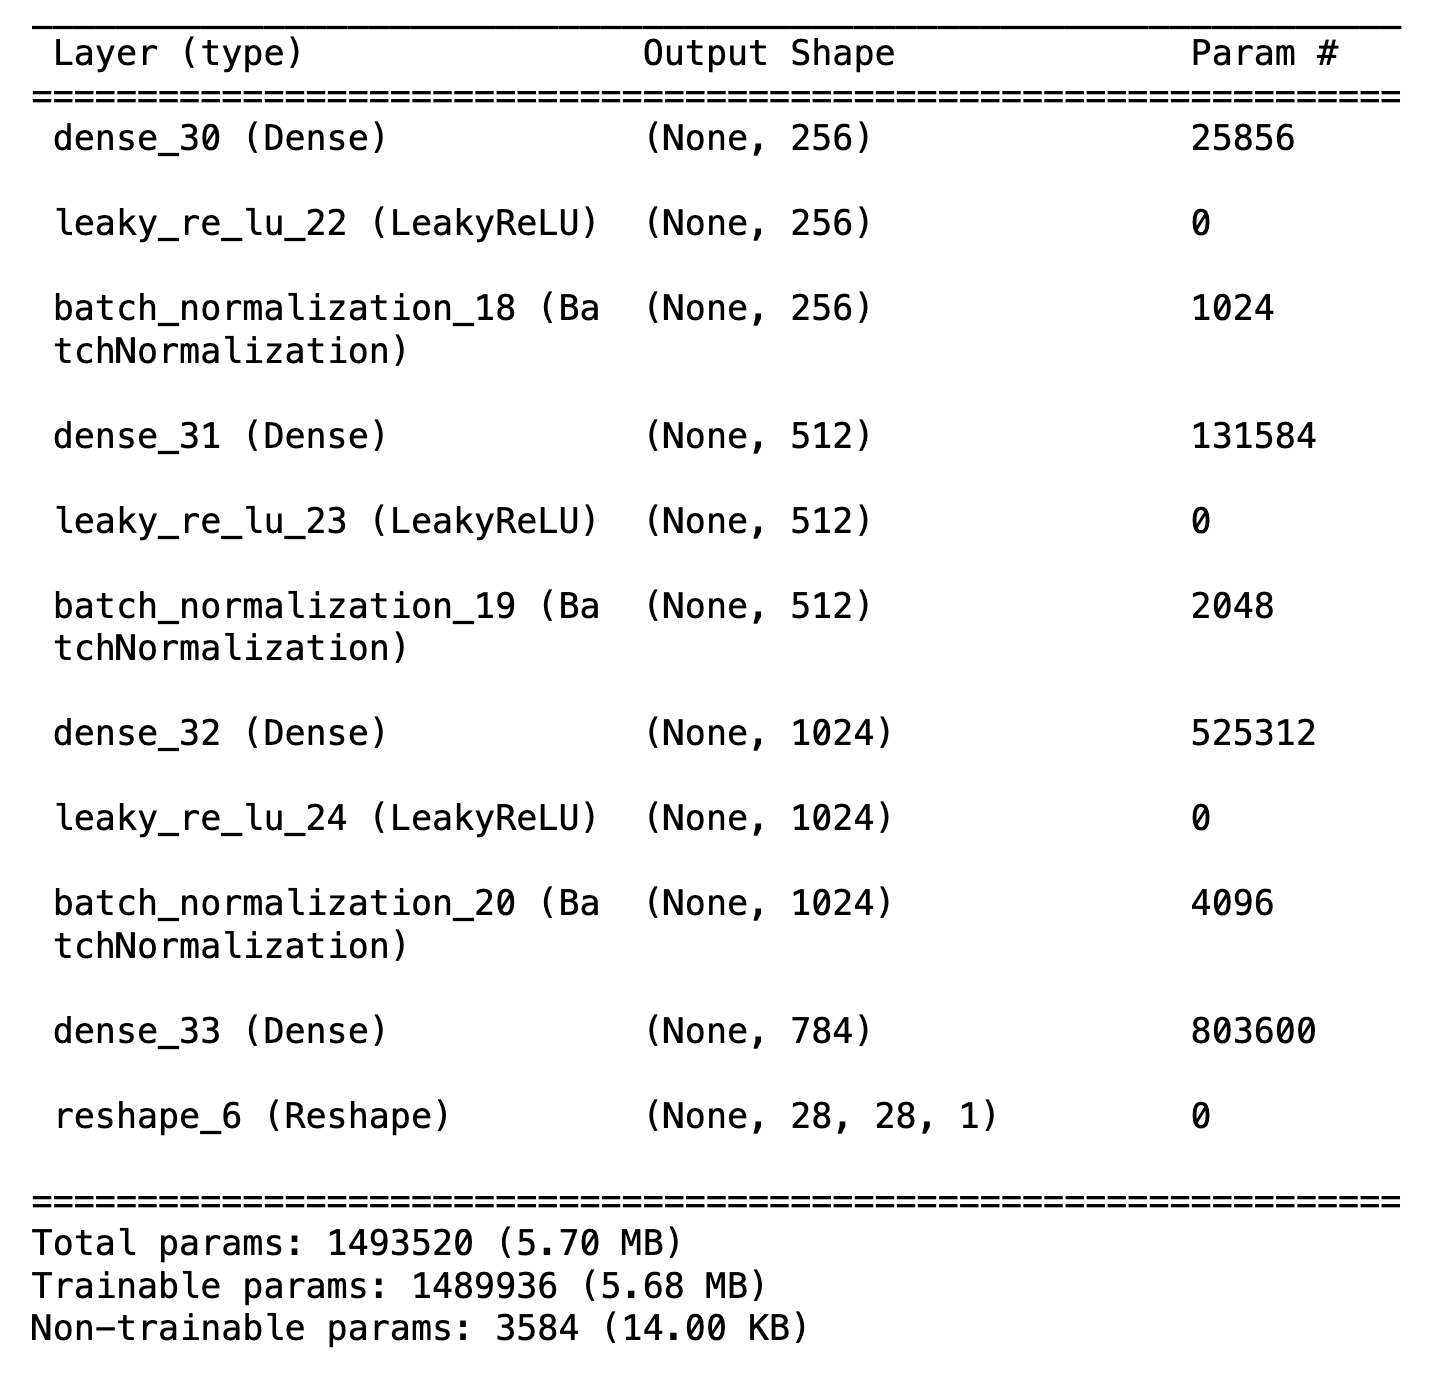
\includegraphics[width=\linewidth]{./Images/generator_dense.jpg}
        \caption{Generator with dense layer}
        \label{fig:Dense}
    \end{subfigure}
    \hspace{0.05\linewidth}
    \begin{subfigure}[b]{0.45\linewidth}
        \centering
        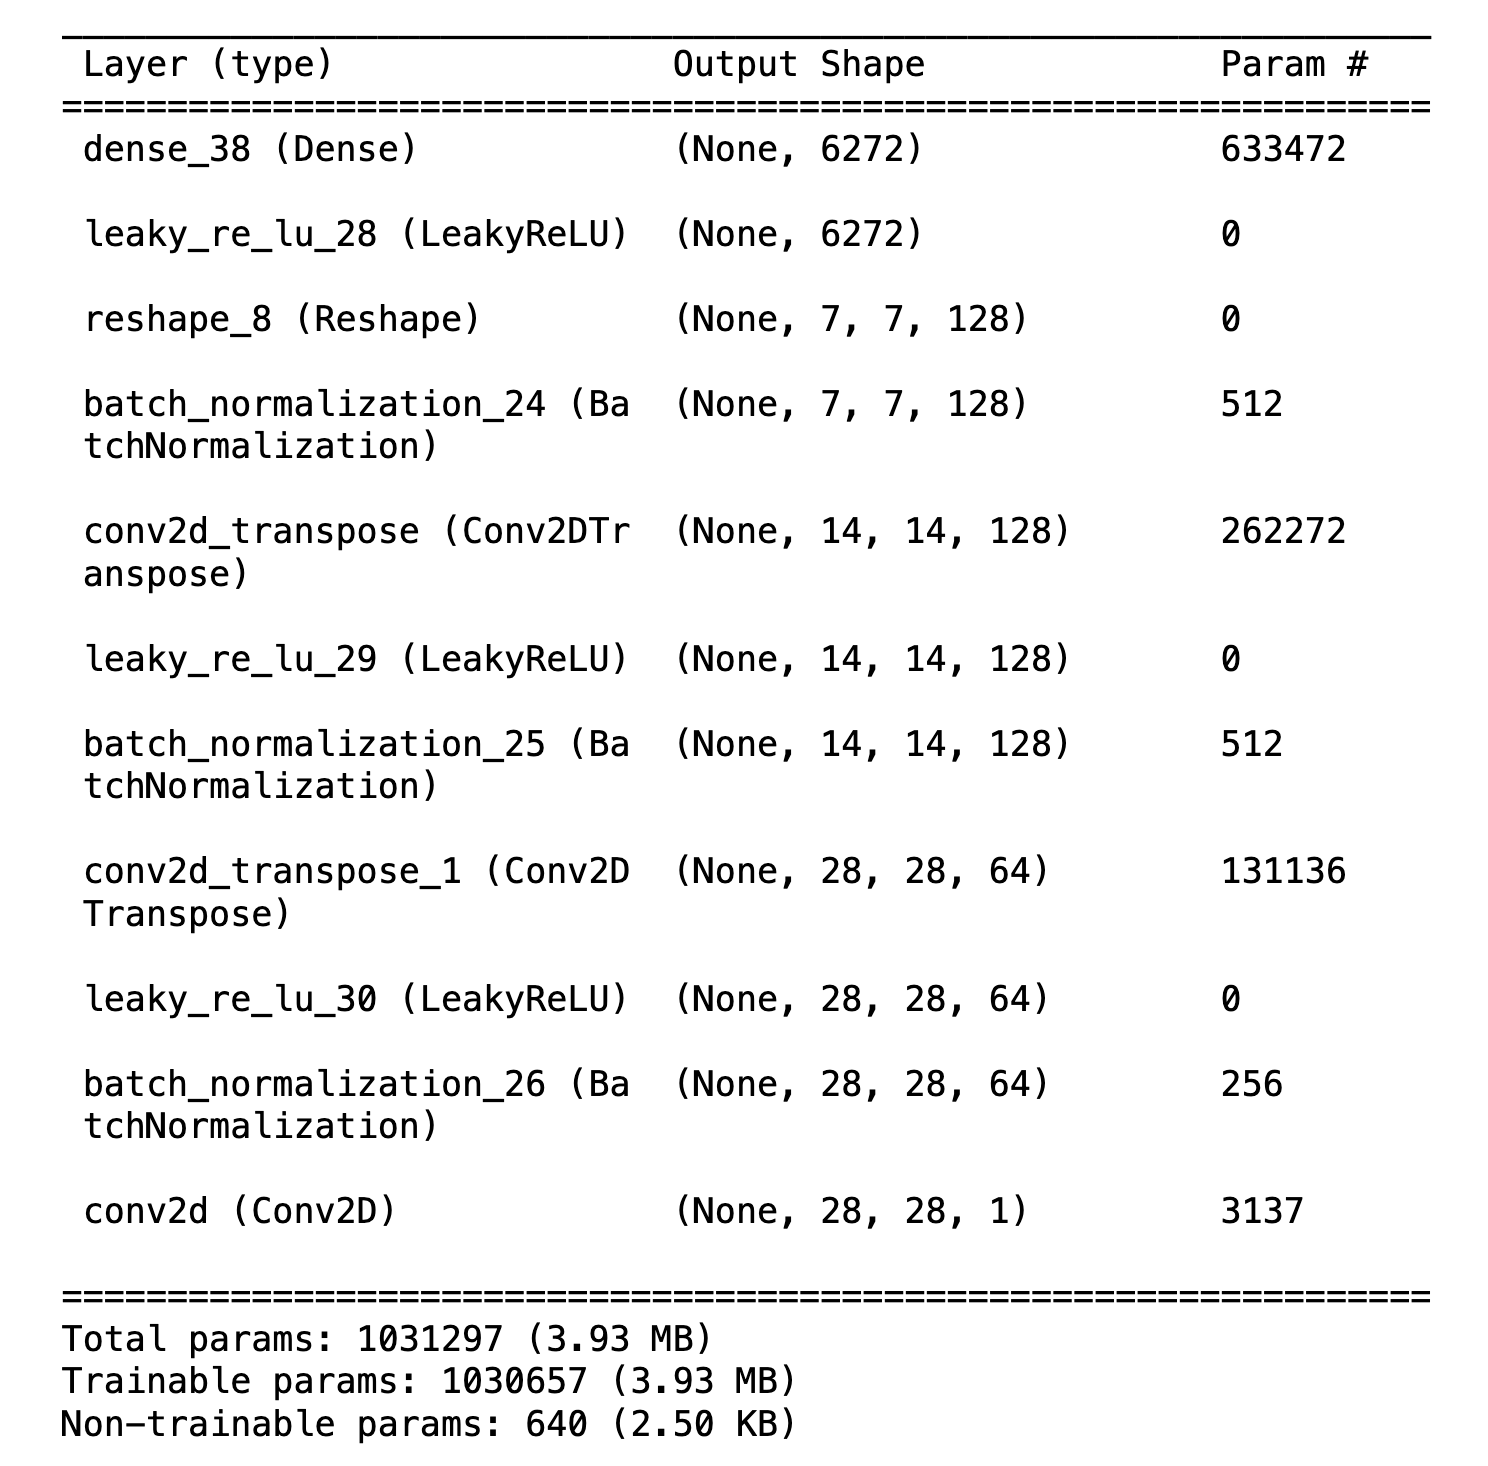
\includegraphics[width=\linewidth]{./Images/generator_cnn.jpg}
        \caption{Generator with convolution layer}
        \label{fig:Conv2D Transpose}
    \end{subfigure}
    \caption{Generator Architecture with Dense and Convolutional Layers}
    \label{fig:combined}
\end{figure}


\begin{figure}[H]
    \centering
    \begin{subfigure}[b]{0.45\linewidth}
        \centering
        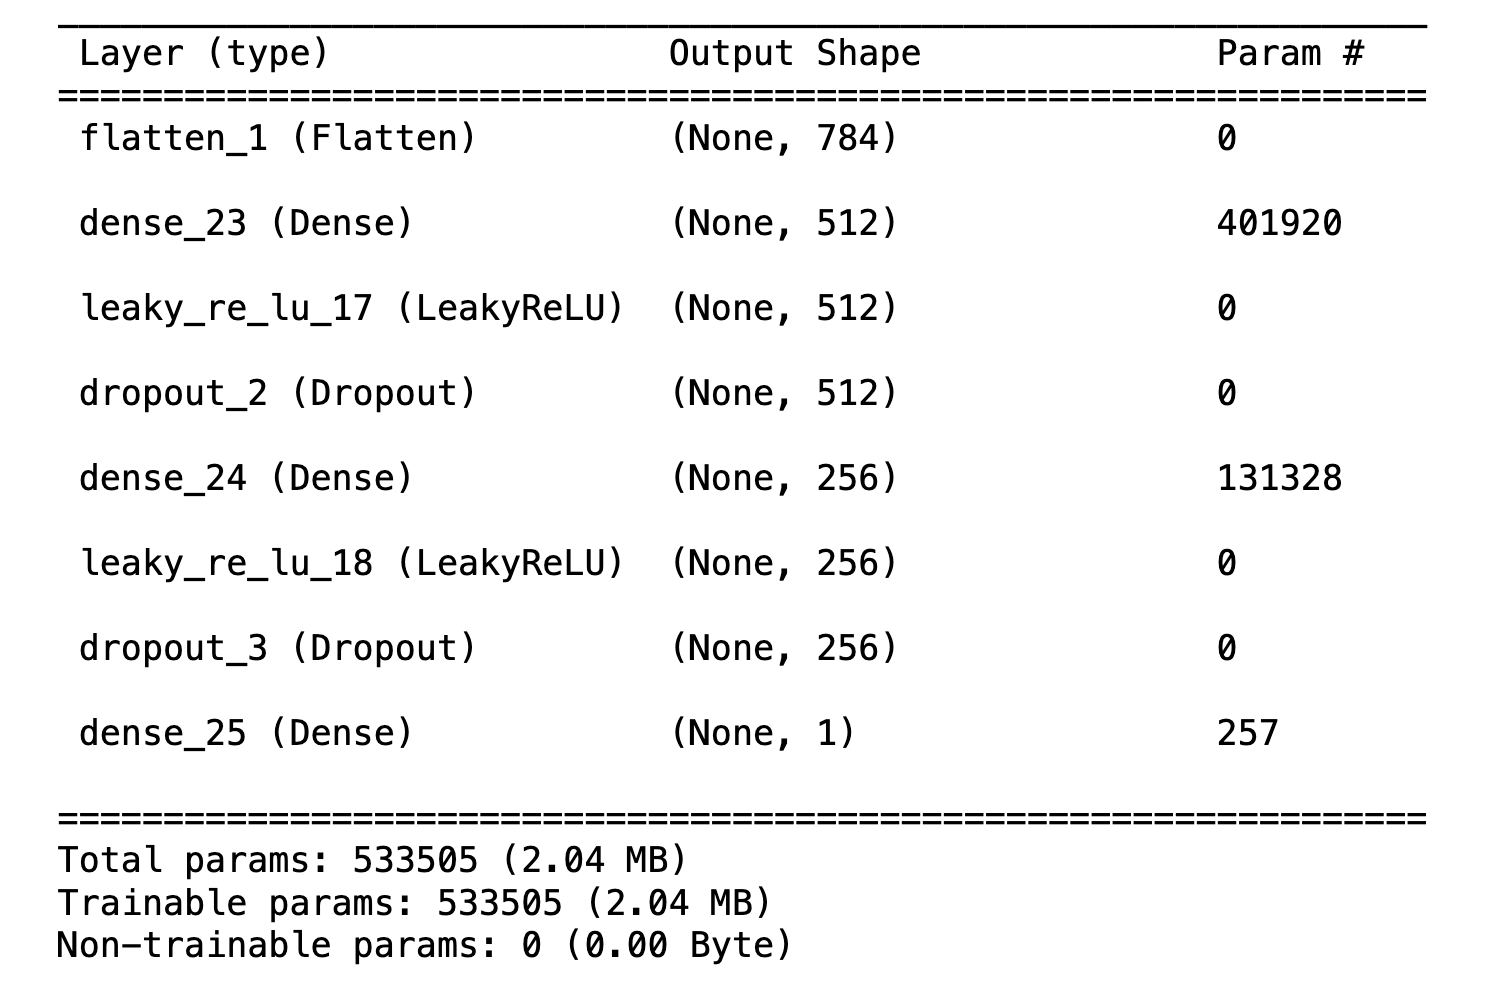
\includegraphics[width=\linewidth]{./Images/discriminator_dense.jpg}
        \caption{Discriminator with dense layer}
        \label{fig:Dense}
    \end{subfigure}
    \hspace{0.05\linewidth}
    \begin{subfigure}[b]{0.45\linewidth}
        \centering
        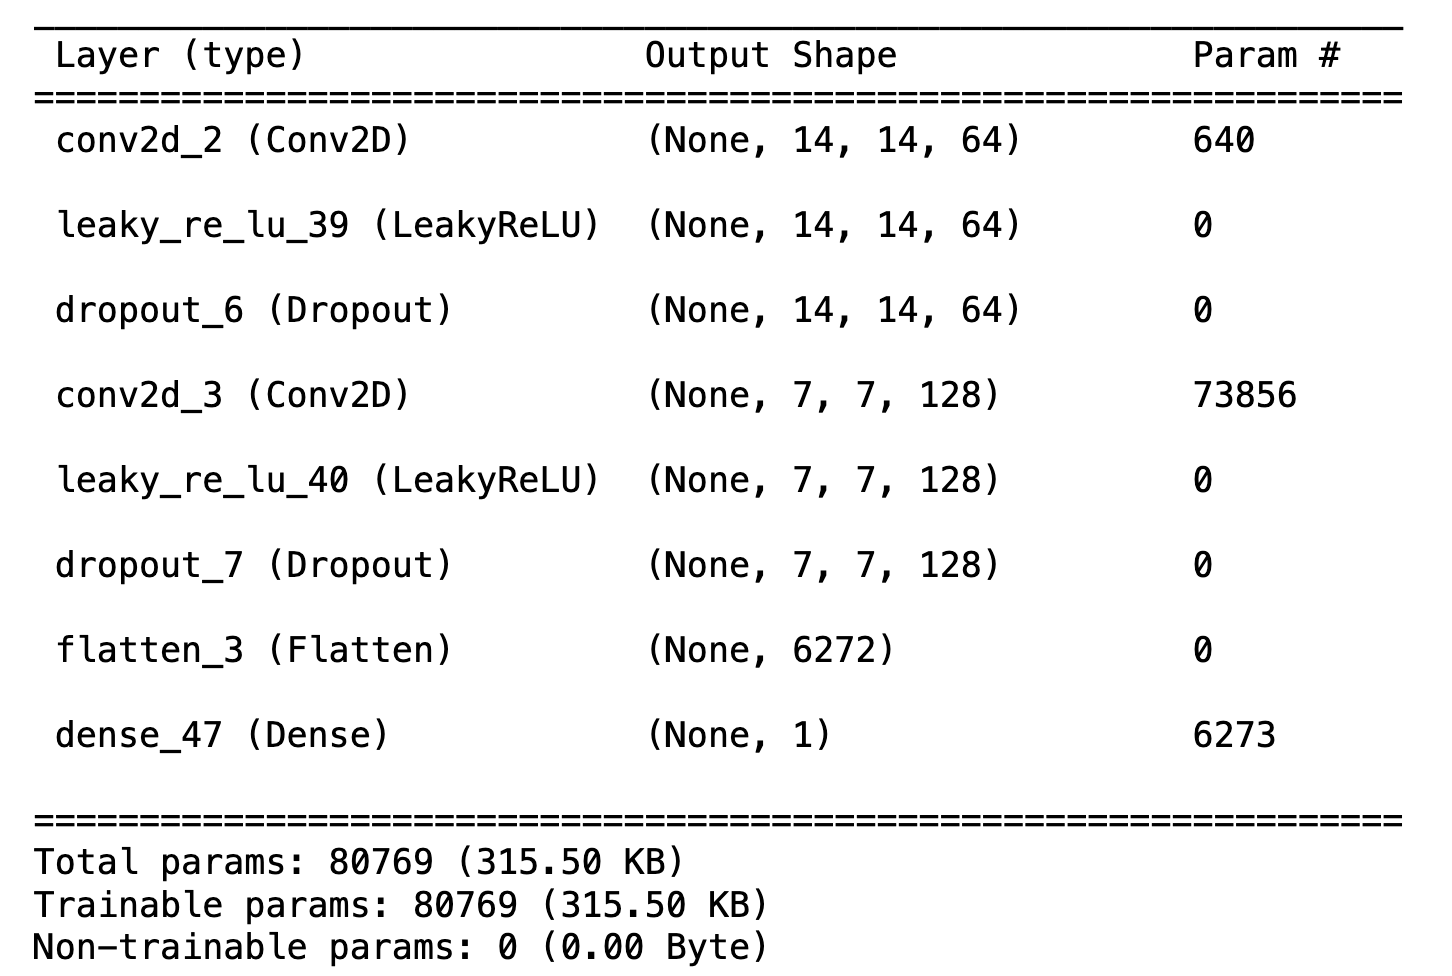
\includegraphics[width=\linewidth]{./Images/discriminator_cnn.jpg}
        \caption{Discriminator with convolution layer}
        \label{fig:Conv2D Transpose}
    \end{subfigure}
    \caption{Discriminator Architecture with Dense and Convolutional Layers}
    \label{fig:combined}
\end{figure}


\begin{figure}[H]
    \centering
    \begin{subfigure}[b]{\linewidth}
        \centering
        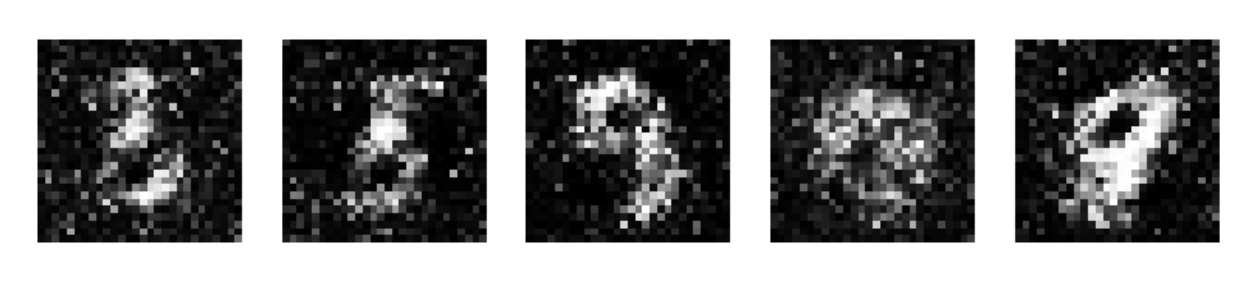
\includegraphics[width=0.7\linewidth]{./Images/generate_image_by_dense_layer.jpg}
        \caption{Images generate by GAN with dense layers}
        \label{fig:Dense}
    \end{subfigure}
    \vspace{0.05\linewidth} 
    \begin{subfigure}[b]{\linewidth}
        \centering
        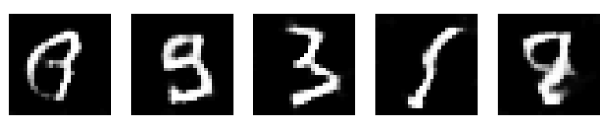
\includegraphics[width=0.7\linewidth]{./Images/generate_image_by_Convolution_layer.jpg}
        \caption{Images generated by GAN with convolution layers}
        \label{fig:Conv2DTranspose}
    \end{subfigure}
    \caption{Comparison of GAN Performance at 3000 Epochs}
    \label{fig:combined}
\end{figure}

\begin{figure}[H]
    \centering
    \begin{subfigure}[b]{\linewidth}
        \centering
        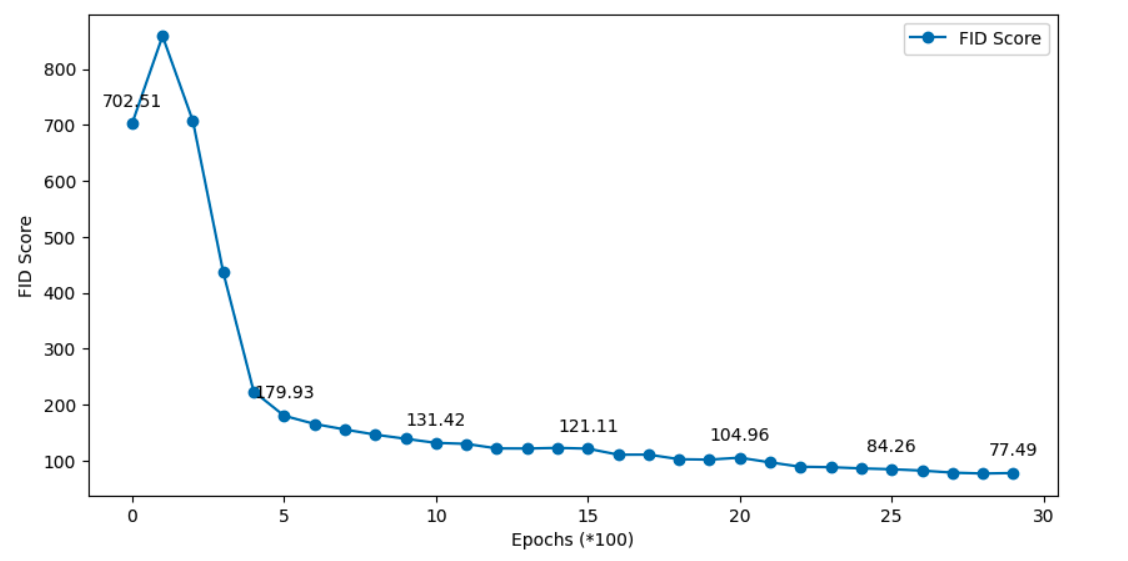
\includegraphics[width=0.7\linewidth]{./Images/fid_score_for_dense_layer.jpg}
        \caption{FID score for dense layer}
        \label{fig:Dense}
    \end{subfigure}
    \vspace{0.05\linewidth} 
    \begin{subfigure}[b]{\linewidth}
        \centering
        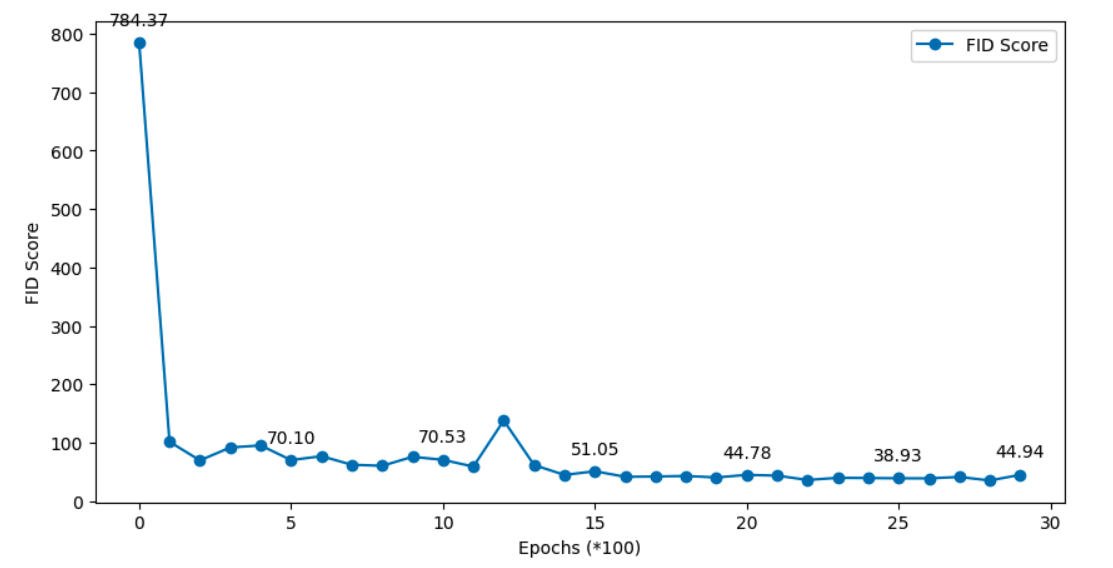
\includegraphics[width=0.7\linewidth]{./Images/fid_score_for_convolution_layer.jpg}
        \caption{FID score for convolutional layer}
        \label{fig:Conv2DTranspose}
    \end{subfigure}
    \caption{FID Scores Across 3000 Epochs}
    \label{fig:combined}
\end{figure}


\section{Exploring Layer Depth}

In this section, I explored the impact of changing convolutional layers in the generator and discriminator of a GAN.

Firstly, I trained the basic convolutional GAN model three times and recorded the FID scores. Secondly, based on the basic structure, I gradually added convolutional layers to the generator, from one to three layers, while keeping the discriminator structure fixed. I trained the model three times for each configuration and recorded the FID scores.

Finally, using the base GAN with three additional convolutional layers in the generator, I gradually added convolutional layers to the discriminator, from one to three layers, while keeping the generator structure fixed. I trained the model three times for each configuration and recorded the FID scores.

Upon comparing, I found that increasing the number of layers in either the generator or the discriminator alone worsened the model’s performance. This imbalance disrupts the dynamic equilibrium between the generator and discriminator in the GAN framework. However, simultaneously increasing the layers in both the generator and the discriminator improved the model’s performance. This finding aligns with the concept of maintaining a balance between the generator and discriminator during training, as highlighted in the literature \citep{10.48550/arxiv.1703.10717}. The importance of this balance is crucial for the effective operation of GANs, ensuring stable learning and improved image quality \citep{10.48550/arxiv.2002.02112}.    

\begin{table}[h]
    \centering
    \caption{FID Scores for Different GAN Architectures (Lower is Better)}
    \begin{tabular}{|l|c|c|c|}
      \hline
      \textbf{GAN Architecture} & \textbf{1st Training} & \textbf{2nd Training} & \textbf{3rd Training} \\
      \hline
      Basic Structure & 68.27 & 76.33 & 59.49 \\
      \hline
      Add 1 Convolution Layer in Generator & 77.25 & 81.14 & 78.46 \\
      \hline
      Add 2 Convolution Layers in Generator & 90.14 & 85.96 & 121.42 \\
      \hline
      Add 3 Convolution Layers in Generator & 151.55 & 147.53 & 284.91 \\
      \hline
      \multicolumn{1}{|l|}{Add 3 Convolution Layers in Generator} & 70.72 & 72.97 & 70.93 \\
      \multicolumn{1}{|l|}{Add 1 Convolution Layer in Discriminator} & & & \\
      \hline
      \multicolumn{1}{|l|}{Add 3 Convolution Layers in Generator} & 37.41 & 42.45 & 31.43 \\
      \multicolumn{1}{|l|}{Add 2 Convolution Layers in Discriminator} & & & \\
      \hline
      \multicolumn{1}{|l|}{Add 3 Convolution Layers in Generator} & 36.75 & 35.87 & 34.72 \\
      \multicolumn{1}{|l|}{Add 3 Convolution Layers in Discriminator} & & & \\
      \hline
    \end{tabular}
    \vspace{2mm}
    \caption*{\textit{Note}: A FID value below 10 is considered to represent very high-quality generated images, 
    while values between 10 and 50 indicate good quality, and values above 50 suggest average or poor quality.}
\end{table}

\begin{figure}[H]
    \centering
    \begin{subfigure}[b]{\linewidth}
        \centering
        \includegraphics[width=0.7\linewidth]{./Images/generate_image_by_convolution_layer.jpg}
        \caption{Images generate by basic structure}
        \label{fig:Dense}
    \end{subfigure}
    \vspace{0.05\linewidth} 
    \begin{subfigure}[b]{\linewidth}
        \centering
        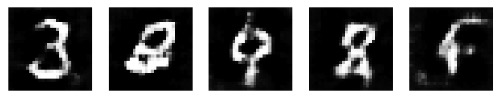
\includegraphics[width=0.7\linewidth]{./Images/both_generator_and_discrimminator_are_add_3_layers.jpg}
        \caption{Images generate by both generator and discriminator are add 3 layers}
        \label{fig:Conv2DTranspose}
    \end{subfigure}
    \caption{Generated Images from Different GAN Architectures}
    \label{fig:combined}
\end{figure}


\section{Impact of Data Augmentation on Model Performance}

I conducted three training runs of the standard GAN model, both with and without data augmentation, 
and compared the FID scores. The results indicate that data augmentation generally led to lower optimization performance.


\begin{figure}[H]
    \centering
    \begin{subfigure}[b]{\linewidth}
        \centering
        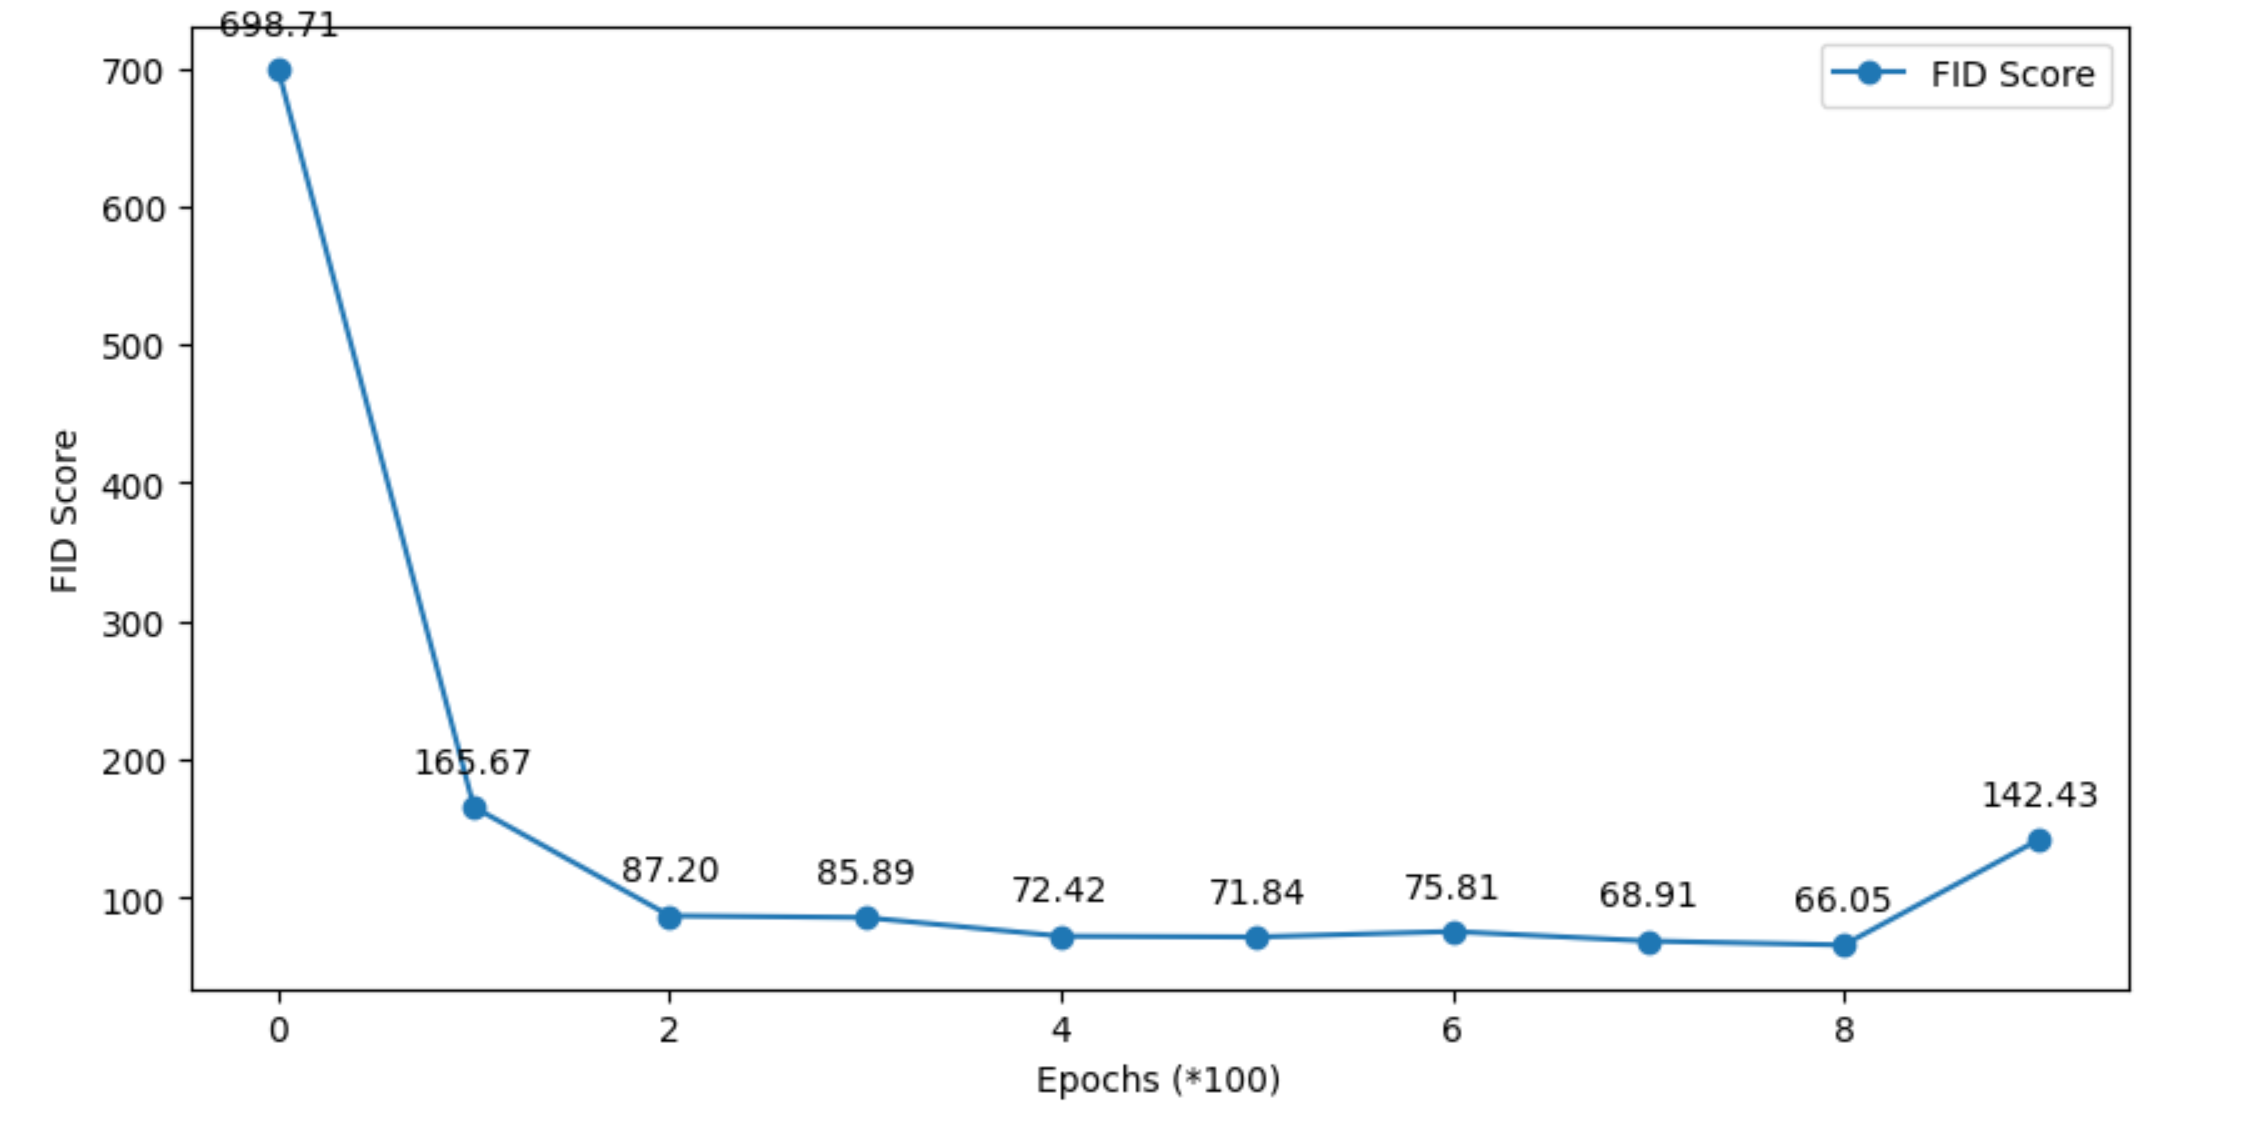
\includegraphics[width=0.8\linewidth]{./Images/standard_GAN_without_data_augementation1.jpg}
        \caption{Standard GAN without data augmentation 1}
        \label{fig:Dense}
    \end{subfigure}
    \vspace{0.05\linewidth} 
    \begin{subfigure}[b]{\linewidth}
        \centering
        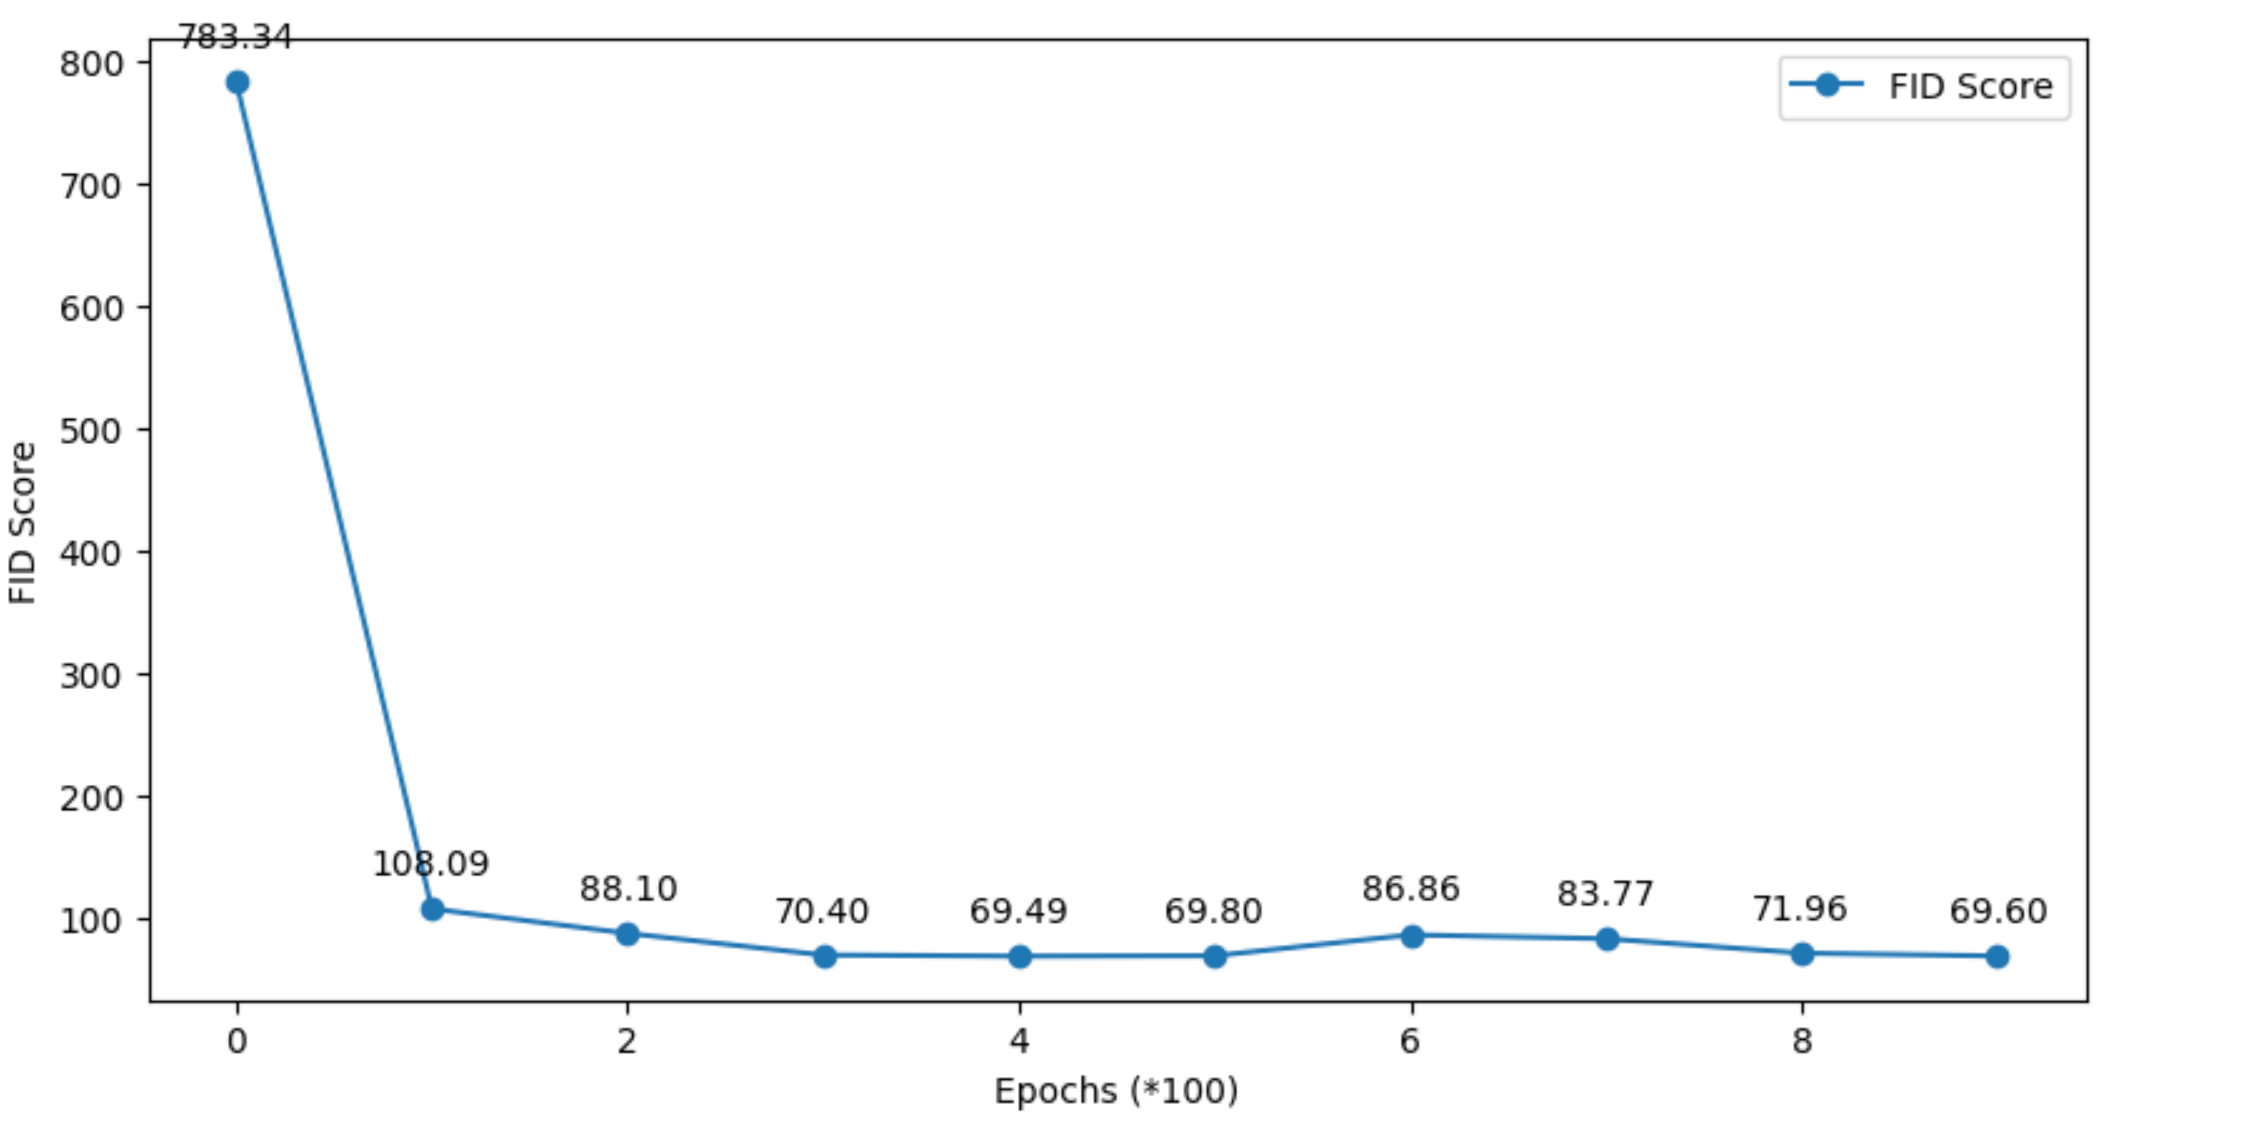
\includegraphics[width=0.8\linewidth]{./Images/standard_GAN_without_data_augementation2.jpg}
        \caption{Standard GAN without data augmentation 2}
        \label{fig:Conv2DTranspose}
    \end{subfigure}
    \begin{subfigure}[b]{\linewidth}
        \centering
        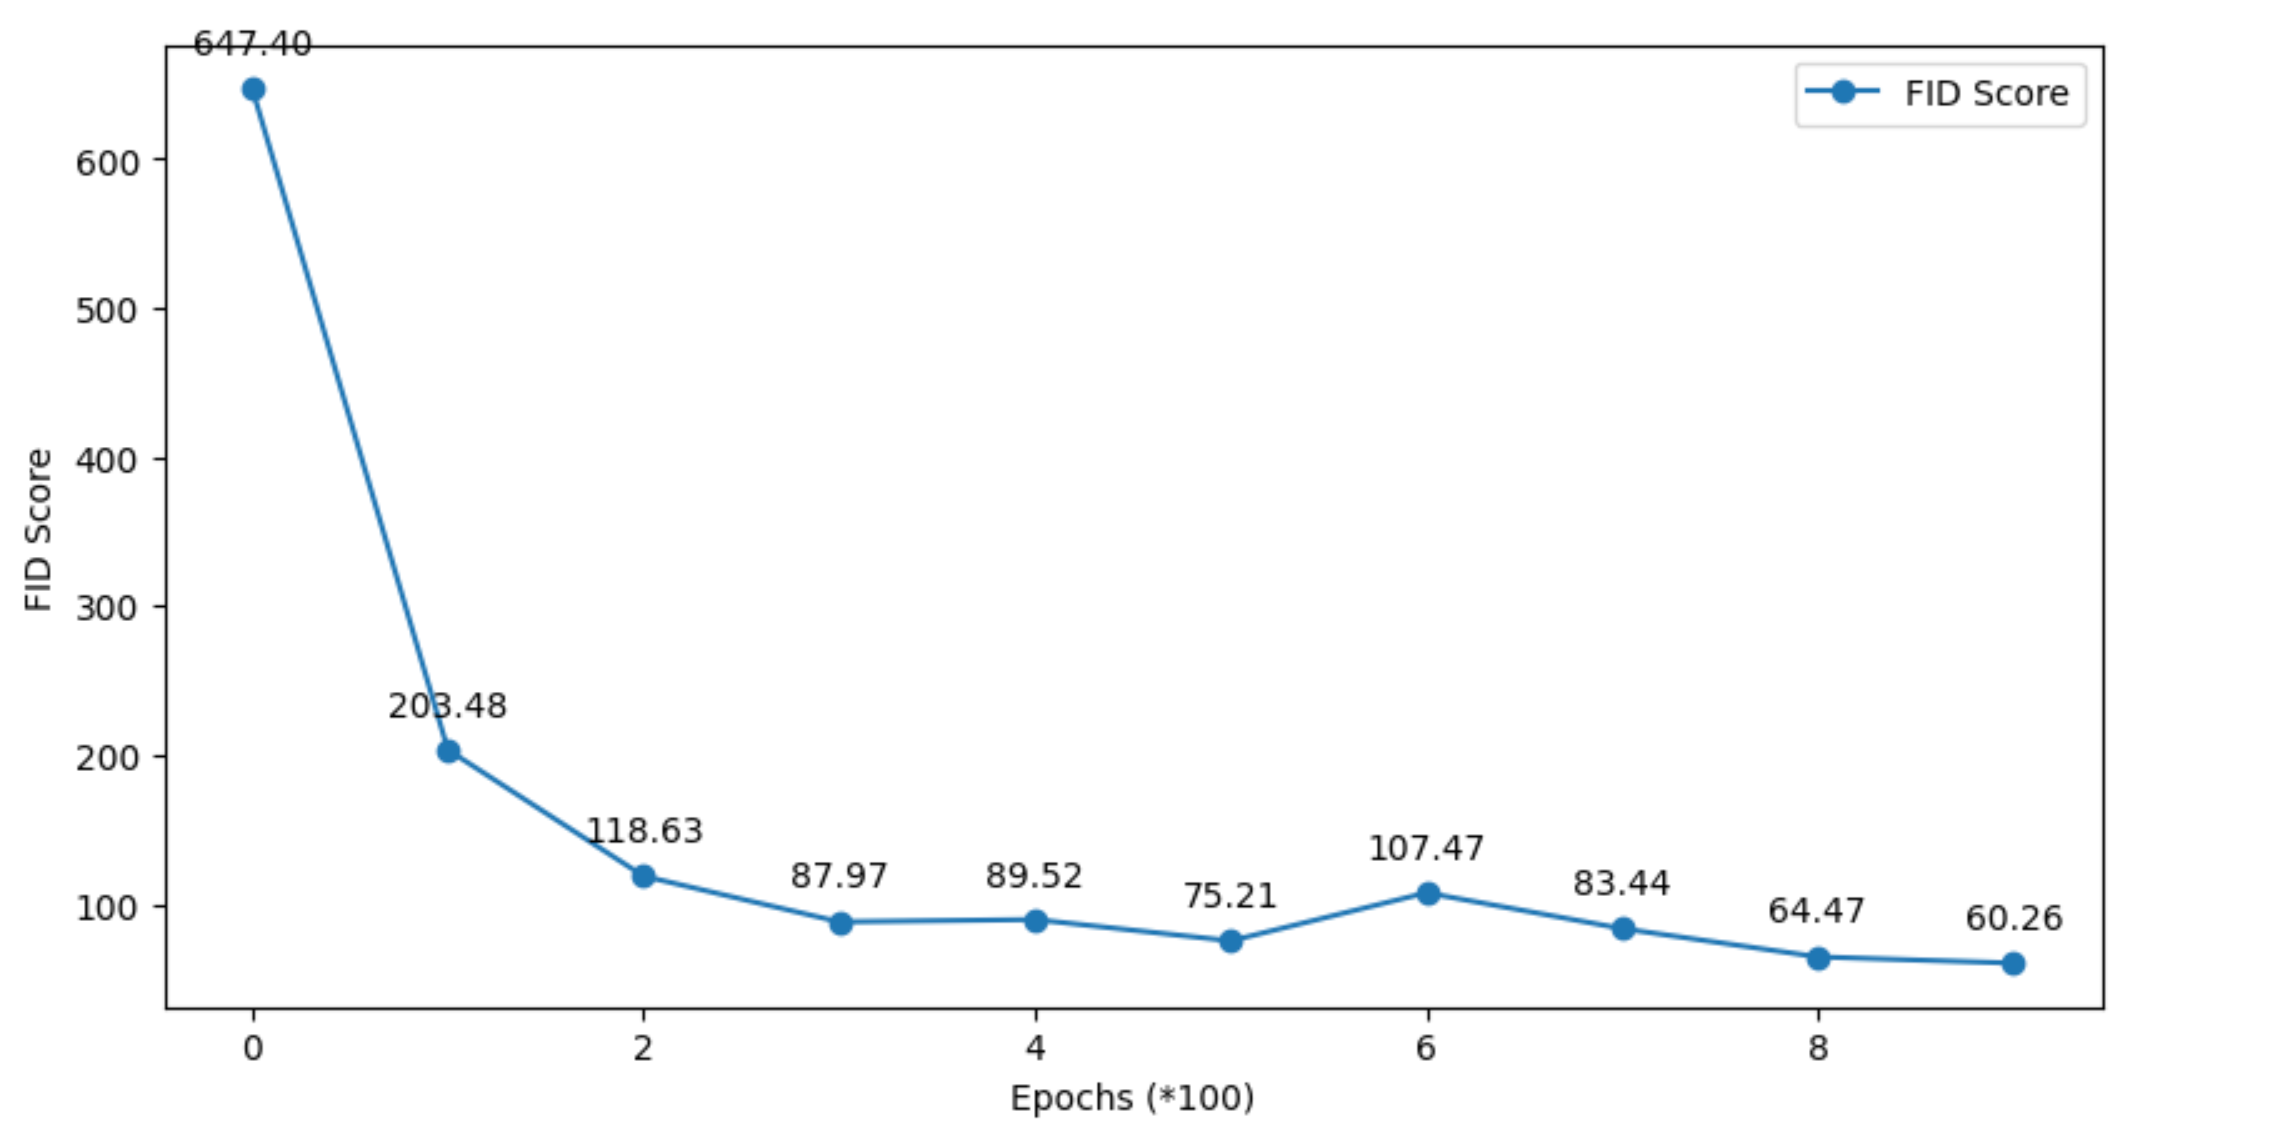
\includegraphics[width=0.8\linewidth]{./Images/standard_GAN_without_data_augementation3.jpg}
        \caption{Standard GAN without data augmentation 3}
        \label{fig:Conv2DTranspose}
    \end{subfigure}
    \caption{The FID scores for standard GAN without data augmentation}
    \label{fig:combined}
\end{figure}


\begin{figure}[H]
    \centering
    \begin{subfigure}[b]{\linewidth}
        \centering
        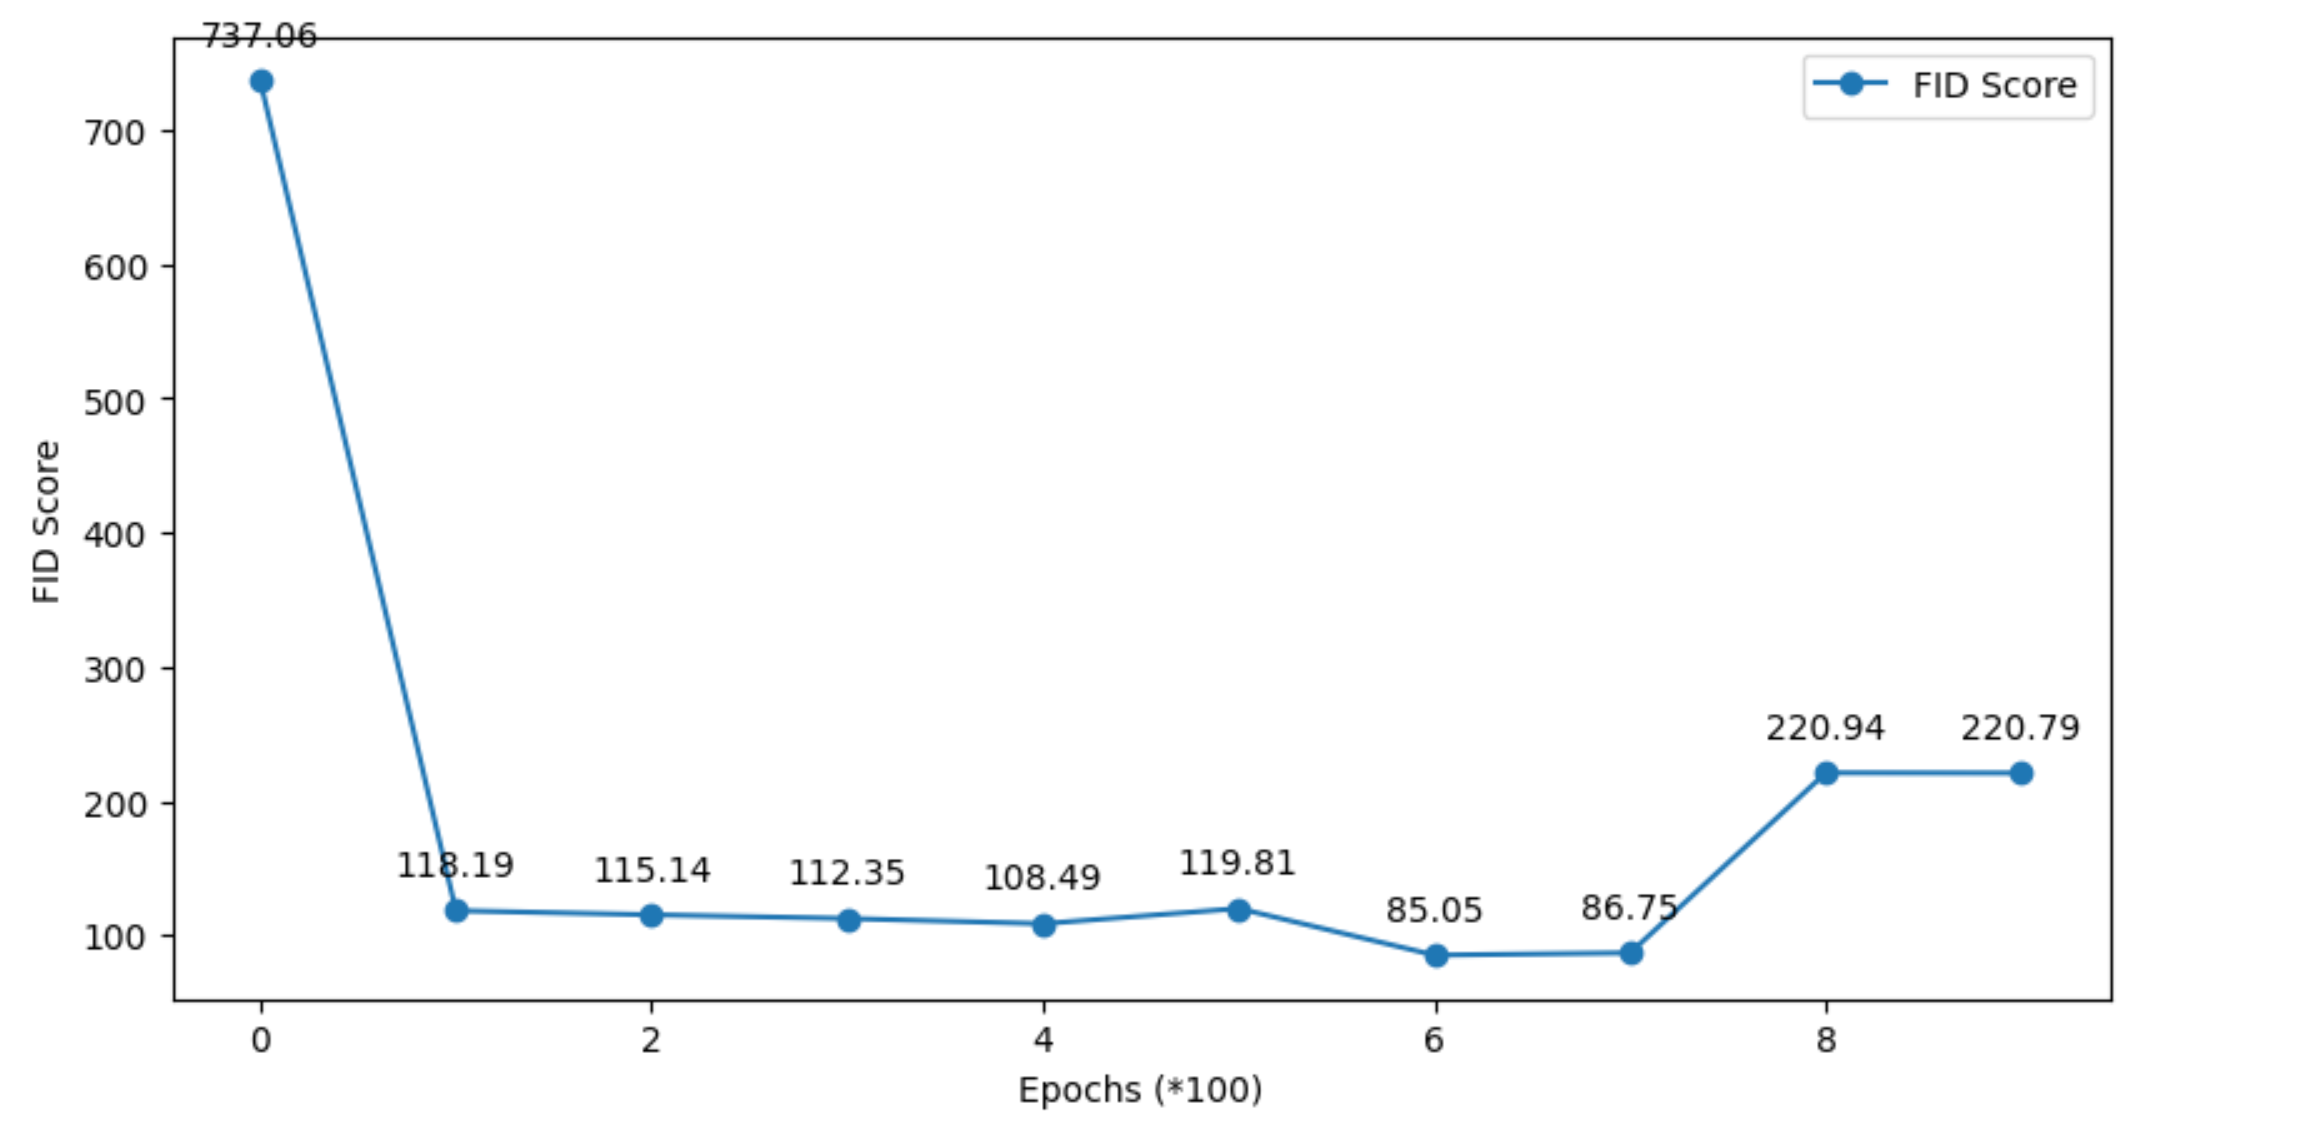
\includegraphics[width=0.84\linewidth]{./Images/standard_GAN_with_data_augementation1.jpg}
        \caption{Standard GAN with data augmentation 1}
        \label{fig:Dense}
    \end{subfigure}
    \vspace{0.05\linewidth} 
    \begin{subfigure}[b]{\linewidth}
        \centering
        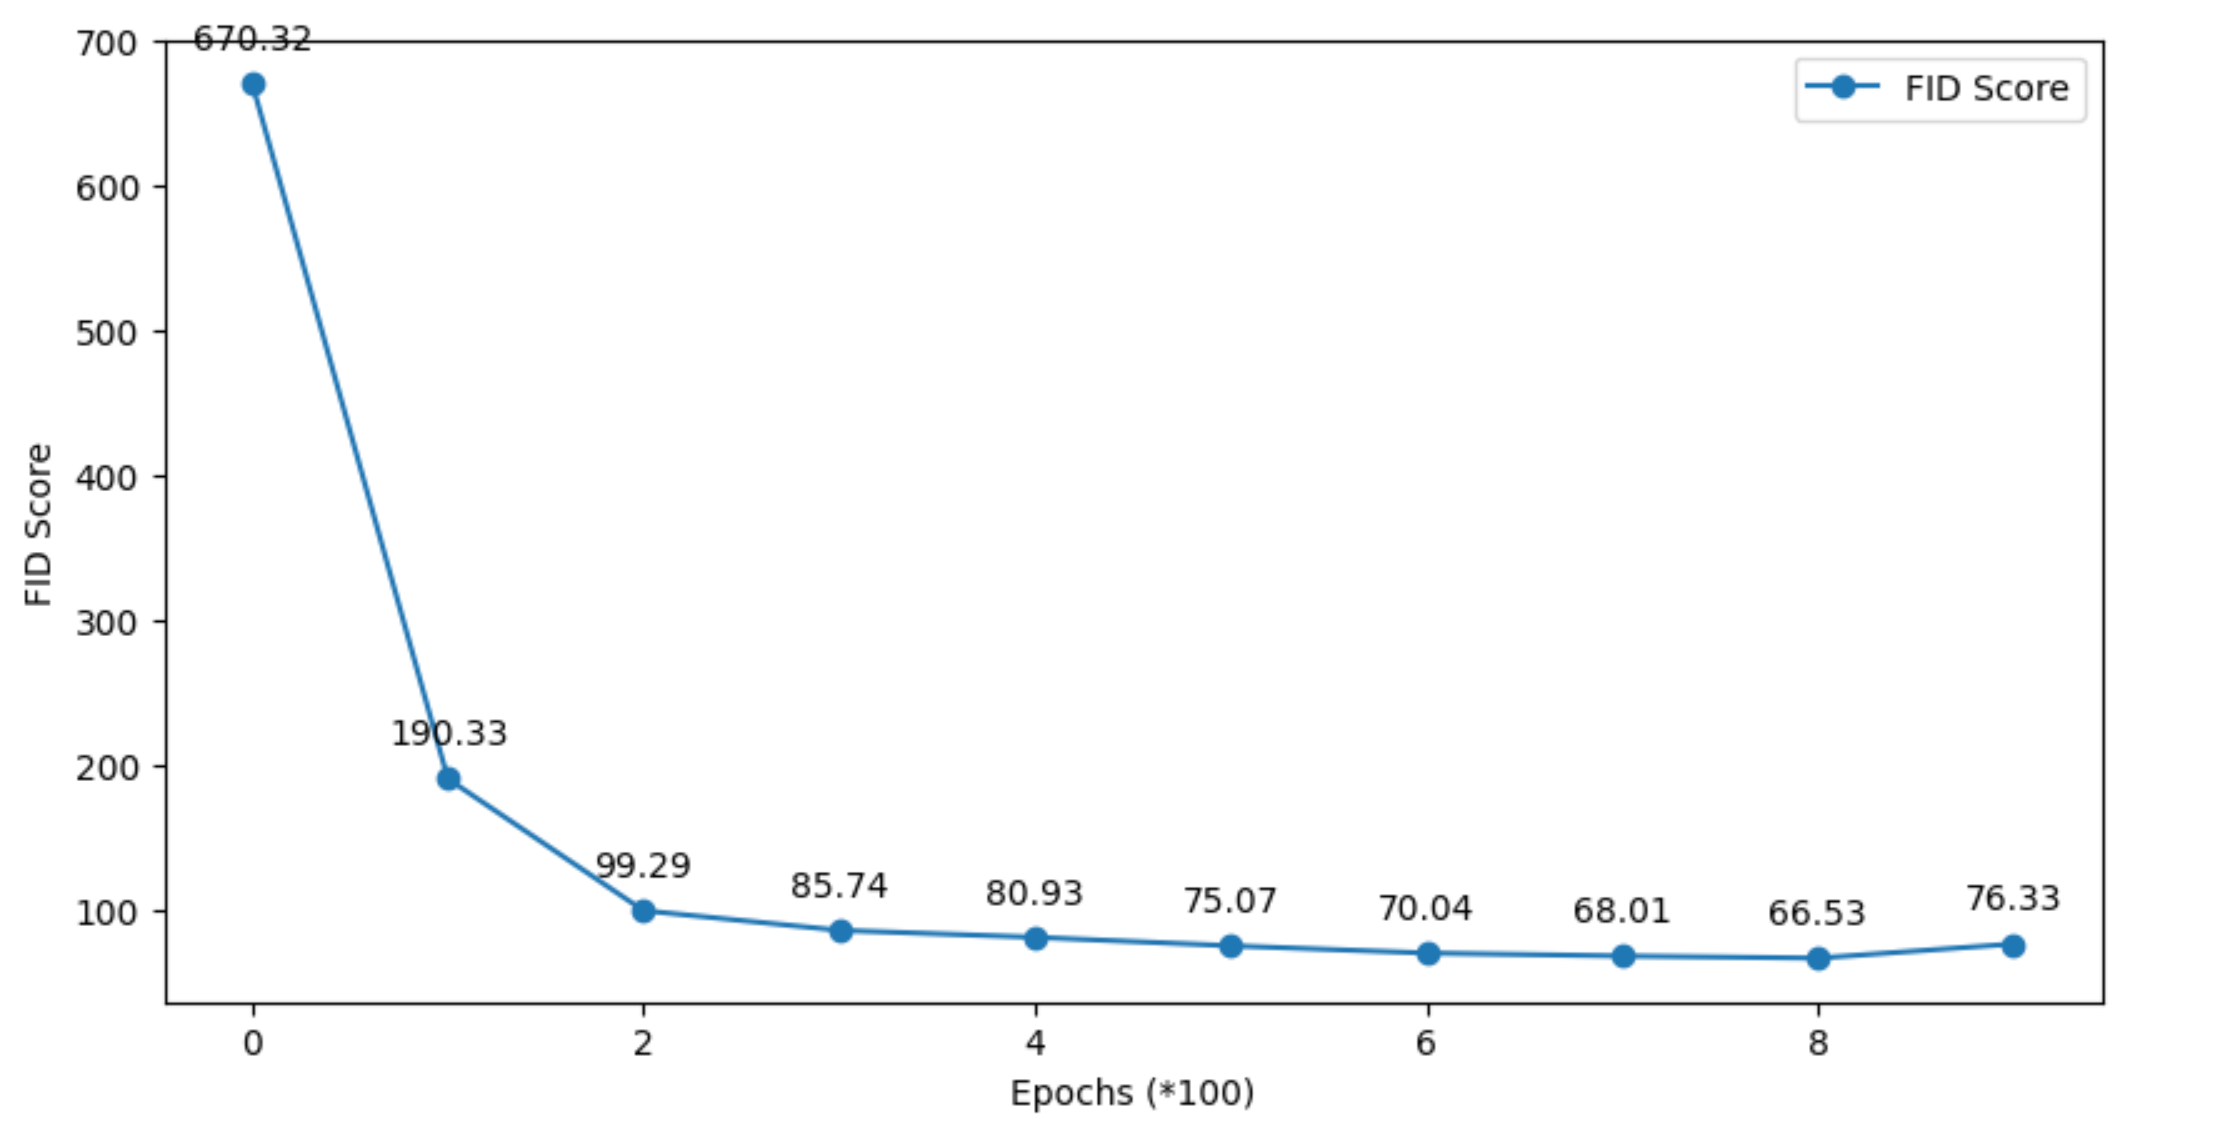
\includegraphics[width=0.8\linewidth]{./Images/standard_GAN_with_data_augementation2.jpg}
        \caption{Standard GAN with data augmentation 2}
        \label{fig:Conv2DTranspose}
    \end{subfigure}
    \begin{subfigure}[b]{\linewidth}
        \centering
        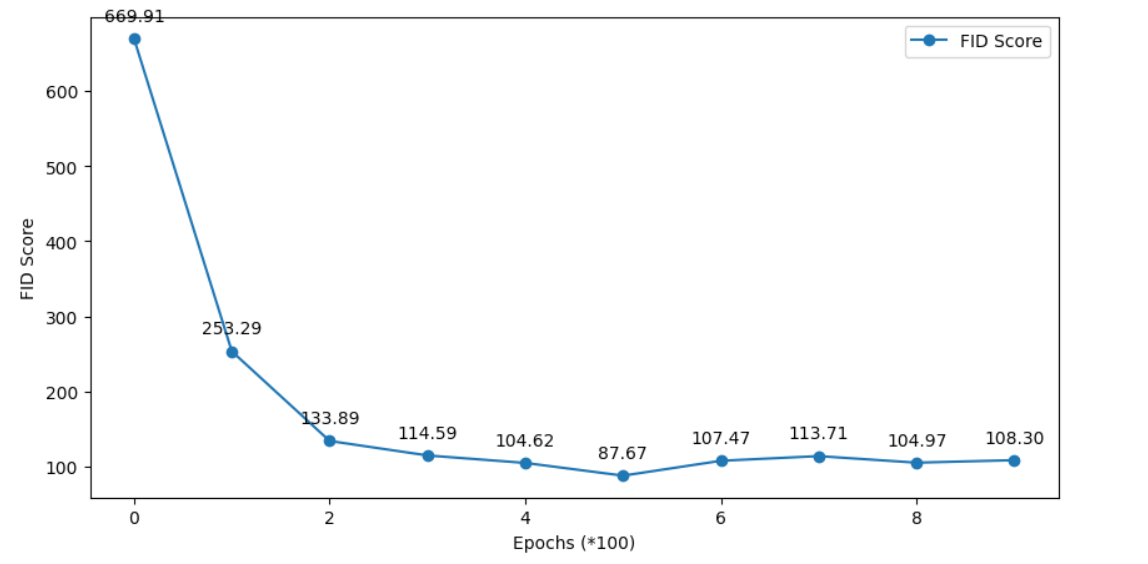
\includegraphics[width=0.8\linewidth]{./Images/standard_GAN_with_data_augementation3.jpg}
        \caption{Standard GAN with data augmentation 3}
        \label{fig:Conv2DTranspose}
    \end{subfigure}
    \caption{The FID scores for standard GAN with data augmentation}
    \label{fig:combined}
\end{figure}

As per usual, the model with data augmentation should performance better then the model without data augmentation.
For why I got this, I think it because of some augmentation technich will disturb the distribution of real image,
this change will mislead the generator to train in the wrong direction.

base on my assumption, I went back to check the code. I have used 4 parameter in data augementation, rotation range, width shift range,
height shift range and horizontal flip.




\section{Applying the Model to a New Dataset}
In this phase, I utilized the Animal Faces-HQ (AFHQ) dataset, which consists of 16,130 high-quality 
images at a resolution of 512x512 pixels, to train a standard GAN model focused on generating realistic 
cat images. Due to the high resolution of the original images, which could potentially cause GPU crashes, 
I downscaled the images to 128x128 pixels. The model was then trained for 4000 epochs. Below are the images 
generated by the model’s generator.


\begin{figure}[h]
    \centering
    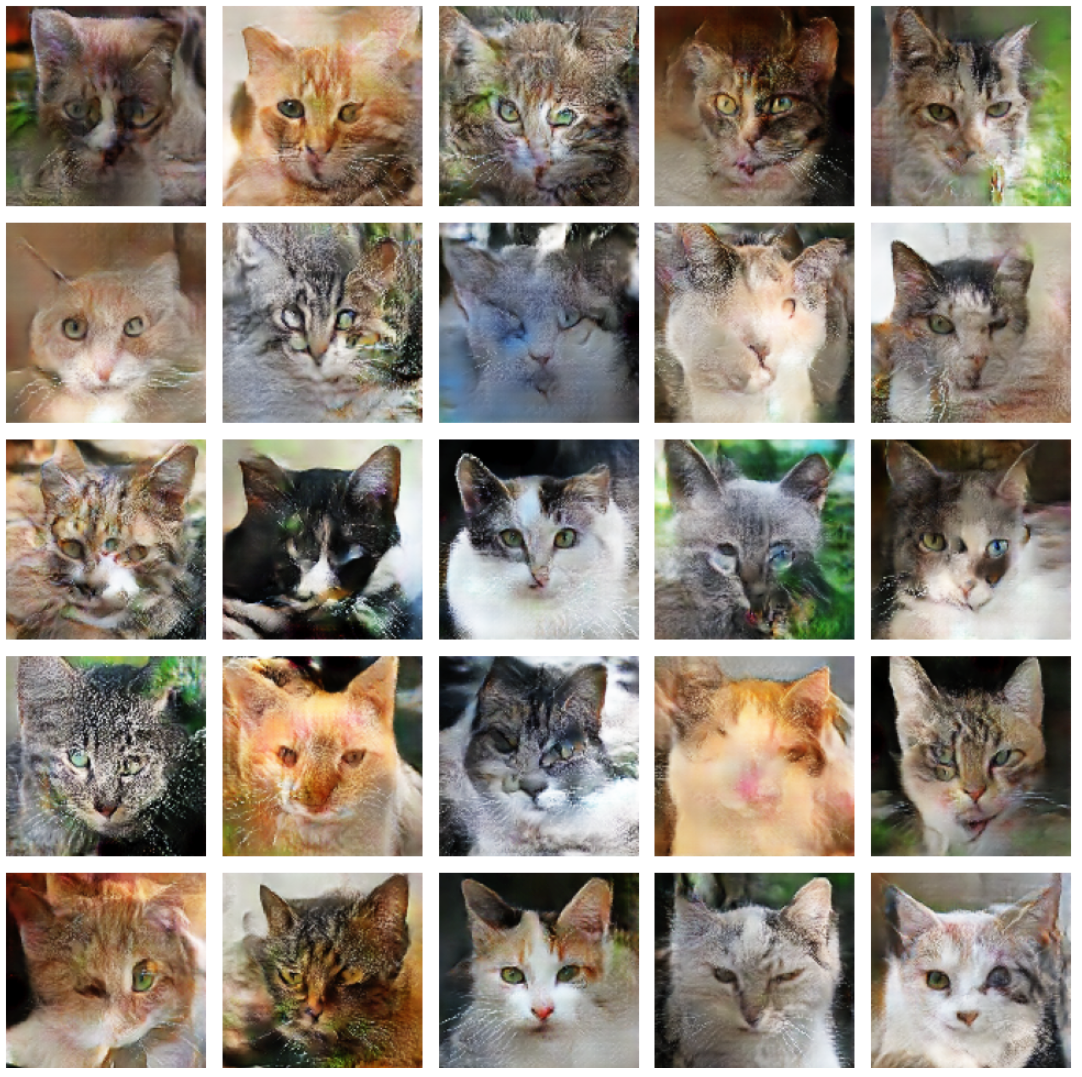
\includegraphics[width=1.0\textwidth]{./Images/apply_new_dataset.jpg} 
    \caption{Cat Faces Generated by GAN}
    \label{fig:apply new dataset}
\end{figure}
